\documentclass{article}

\usepackage[preprint]{neurips_2024}

\usepackage[utf8]{inputenc}
\usepackage[T1]{fontenc}
\usepackage{hyperref}
\usepackage{url}
\usepackage{booktabs}
\usepackage{amsfonts}
\usepackage{amsmath}
\usepackage{amssymb}
\usepackage{nicefrac}
\usepackage{microtype}
\usepackage{graphicx}
\usepackage{xcolor}
\usepackage{tikz}
\usetikzlibrary{arrows.meta, positioning, fit, calc, shapes.geometric}
\usepackage{placeins}

% keep floats close to their references
\renewcommand{\topfraction}{0.92}
\renewcommand{\bottomfraction}{0.85}
\renewcommand{\textfraction}{0.07}
\renewcommand{\floatpagefraction}{0.80}
\setcounter{topnumber}{3}
\setcounter{bottomnumber}{2}
\setcounter{totalnumber}{5}

\title{Inference-Time Safety Guidance for Diffusion Models:\\
A Tunable Pareto Knob via Classifier-Energy on the Tweedie Estimate}

\author{%
  Boyu Yang \quad Luojia Xia \quad William Zhang \quad Vincent Lin \\
  Department of Computer Science \\
  Yale University \\
}

\begin{document}

\maketitle

\begin{abstract}
Text-to-image diffusion models continue to generate violent, explicit, and otherwise unsafe imagery, even from prompts that look benign on the surface. Retraining the model away from such content is expensive and locks in a single safety policy. We study a purely inference-time alternative: at every denoising step, the predicted clean image is decoded, scored by a frozen safety classifier, and a hinge-energy gradient is back-propagated through the decoder into the latent. The strength of the correction is governed by a single scalar knob $\lambda$. We compare this construction against four baselines---vanilla sampling, negative prompts, Safe Latent Diffusion, and rejection sampling---on a stratified benchmark of 875 prompts spanning six hazard categories. The classifier-energy method traces a smooth safety--quality Pareto frontier as $\lambda$ varies and is the only baseline that pushes the unsafe rate below five percent on the explicit stratum, where an architecturally disjoint NudeNet evaluator confirms the ranking (Spearman~$\rho=0.93$). Negative prompting, by contrast, dominates at moderate safety levels and runs three times faster. We argue that any new inference-time defense should be calibrated against this trade-off rather than reported in isolation.
\end{abstract}

\section{Introduction}
\label{sec:intro}

Stable Diffusion and its descendants are now deployed at scale, and the cost of unsafe outputs is no longer hypothetical. The I2P benchmark~\citep{schramowski2023sld} showed that off-the-shelf SD~1.5 produces violent or sexually explicit content for a non-trivial fraction of even ostensibly innocuous prompts; subsequent jailbreak suites~\citep{yang2024mma,tsai2024ringabell} demonstrated that adversarial prompts can elicit such content reliably. Industry response has split along two lines.

The first line, model-level concept erasure, fine-tunes the U-Net so that target concepts are no longer accessible~\citep{gandikota2023esd,kumari2023ablation}. This is effective but expensive: each new policy requires another optimization pass, the resulting weights are static, and there is no way to dial safety up or down at inference time. Downstream users inherit whatever trade-off the model owner committed to.

The second line, inference-time guidance, leaves the weights frozen and biases the sampling trajectory. Negative prompts subtract a hard-coded text embedding from classifier-free guidance~\citep{ho2022cfg}; Safe Latent Diffusion (SLD,~\citealp{schramowski2023sld}) generalizes this with a momentum term and a thresholded mask. Rejection sampling at the output of the decoder is also commonly used as a last-mile filter. These methods are cheap and modular, but each has a structural shortcoming: negative prompts are essentially binary, SLD's defaults are tuned conservatively and barely move the needle on our benchmark, and rejection wastes compute on samples that are then discarded.

We revisit a third option that has been less explored in the safety setting: classifier guidance~\citep{dhariwal2021diffusion}. The new ingredient is to evaluate the classifier not on the noisy latent (where it is uninformative) but on the Tweedie estimate $\hat{x}_0$~\citep{efron2011tweedie,bansal2023universal}---an explicit prediction of the clean image at the current step---and to add the resulting gradient to the DDIM update. The strength is controlled by a single scalar~$\lambda$. Our contributions are:

\begin{itemize}
\item A classifier-energy guidance term operating on the Tweedie estimate, with a continuous strength knob that traces a smooth Pareto curve between unsafe rate and prompt fidelity.
\item A head-to-head comparison of five method families (vanilla, negative prompt, SLD, rejection, classifier-energy at four $\lambda$ values plus two fixed-schedule ablations) on a stratified 875-prompt benchmark across six hazard categories.
\item Cross-evaluator validation on the explicit stratum using NudeNet, an architecturally disjoint detector, which agrees with our CLIP evaluator at $\rho=0.93$ and rules out circular-evaluation artifacts as the explanation for the observed ordering.
\end{itemize}

The honest takeaway is not that classifier-energy guidance dominates everything. At moderate safety, plain negative prompting is more cost-effective; classifier-energy earns its place by extending the Pareto curve into a strict-safety regime that no other inference-time baseline reaches.

\section{Background and Related Work}
\label{sec:background}

\paragraph{Diffusion sampling.} A latent diffusion model~\citep{rombach2022ldm} learns a denoising network $\epsilon_\theta(z_t, c)$ which, given a noisy latent $z_t$ at timestep $t$ and conditioning $c$, predicts the noise component. Deterministic sampling via DDIM~\citep{song2021ddim} iterates
\begin{equation}
z_{t-1} = \sqrt{\bar\alpha_{t-1}}\,\hat{z}_0(z_t) + \sqrt{1-\bar\alpha_{t-1}}\,\epsilon_\theta(z_t, c),
\qquad
\hat{z}_0(z_t) = \frac{z_t - \sqrt{1-\bar\alpha_t}\,\epsilon_\theta(z_t, c)}{\sqrt{\bar\alpha_t}},
\label{eq:ddim}
\end{equation}
where $\hat{z}_0$ is the Tweedie estimate of the clean latent, exposed at every step as a side effect of the denoising. Classifier-free guidance~\citep{ho2022cfg} mixes a conditional and unconditional noise prediction; classifier guidance~\citep{dhariwal2021diffusion} adds the gradient of an external classifier.

\paragraph{Inference-time safety baselines.} \emph{Negative prompts} subtract the noise prediction conditioned on a hand-written textual concept (e.g., ``nudity, blood, weapons'') from the conditional branch of CFG. \emph{Safe Latent Diffusion}~\citep{schramowski2023sld} adds momentum and a thresholded mask to the negative direction. \emph{Rejection sampling} regenerates a sample (up to a cap) when a post-hoc filter flags it as unsafe. All three are implemented on the same DDIM loop in our experiments.

\paragraph{Universal guidance.} \citet{bansal2023universal} use the Tweedie estimate $\hat{x}_0$ as the input to an off-the-shelf classifier during diffusion sampling, with applications to style, segmentation, and face identity. We instantiate the same primitive for safety, and characterize its trade-off against the standard inference-time defenses.

\paragraph{Evaluation hygiene.} A recurring pitfall in this literature is using the same CLIP encoder for both guidance and evaluation, which inflates the reported safety. We use OpenAI ViT-B/32 for guidance and ViT-L/14 for evaluation, with NudeNet~\citep{nudenet}---an ONNX CNN trained on entirely different data---as a third party.

\paragraph{Training-time alternatives.} A separate line of work fine-tunes the diffusion weights to remove unsafe concepts---e.g., Erased Stable Diffusion~\citep{gandikota2023esd} and concept ablation~\citep{kumari2023ablation}. These approaches are complementary to ours; we focus on inference-time control because it leaves the weights untouched and exposes a runtime knob to downstream users.

\section{Method}
\label{sec:method}

\subsection{Single-loop sampler}
All five method families share one DDIM loop; methods differ only in a guidance hook applied either before the noise prediction (modifying $\epsilon_\theta$) or after it (correcting $z_{t-1}$). This keeps the comparison apples-to-apples: wall-clock numbers and Pareto positions reflect the algorithm rather than incidental implementation differences.

\subsection{Classifier-energy guidance on $\hat{x}_0$}

Let $c_\phi(\cdot) \in [0,1]$ be a frozen safety classifier returning the cosine similarity between an image and an unsafe-concept embedding. We define the hinge energy
\begin{equation}
L_{\mathrm{unsafe}}(x) = \sum_{k=1}^{K} w_k\,\max\bigl(0,\; c_\phi^{(k)}(x) - \tau\bigr),
\label{eq:hinge}
\end{equation}
summed over $K=7$ unsafe concepts (nudity, blood, weapons, gore, hate symbols, drugs, self-harm). The hinge ensures that benign content (already below threshold) contributes no gradient.

At each step we form the Tweedie estimate $\hat{z}_0$ via Eq.~\ref{eq:ddim}, decode $\hat{x}_0 = \mathcal{D}(\hat{z}_0)$ through the (frozen) VAE, evaluate $L_{\mathrm{unsafe}}(\hat{x}_0)$, and back-propagate to $z_t$. The corrected DDIM update is
\begin{equation}
z_{t-1} \leftarrow \mathrm{DDIM}\bigl(z_t,\,\epsilon_\theta(z_t, c)\bigr) \;-\; \lambda_t \,\nabla_{z_t} L_{\mathrm{unsafe}}\bigl(\hat{x}_0(z_t)\bigr).
\label{eq:correct}
\end{equation}
Two implementation details matter. First, the U-Net forward pass that produces $\hat{z}_0$ must be re-executed under autograd; the cached $\epsilon_\theta$ from the no-grad branch cannot be reused. Second, the VAE runs in fp16 by default, but the cumulative-$\bar\alpha$ scalars used in Eq.~\ref{eq:ddim} live in fp32; mixing the two without explicit casts produces silent NaNs in the gradient.

\paragraph{Adaptive schedule.} A fixed $\lambda$ over-steers when the prompt is already safe and under-steers when it is not. We modulate
\begin{equation}
\lambda_t = \lambda_0 \cdot \sigma\!\left(\beta\,\bigl[\max_k c_\phi^{(k)}(\hat{x}_0) - \tau\bigr]\right) \cdot \mathbf{1}[t \in [t_{\min}, t_{\max}]],
\label{eq:adaptive}
\end{equation}
so that guidance ramps up in proportion to the violation margin and is restricted to a mid-to-late timestep window where $\hat{x}_0$ has converged enough to be informative ($[15, 40]$ of 50 steps in our experiments). We compare against a fixed-$\lambda$ ablation in Section~\ref{sec:results}.

\subsection{Schematic}

Figure~\ref{fig:schematic} summarizes the loop. The guidance branch on the right is what distinguishes our method from a vanilla DDIM step (top row).

\begin{figure}[htbp]
\centering
\resizebox{\linewidth}{!}{%
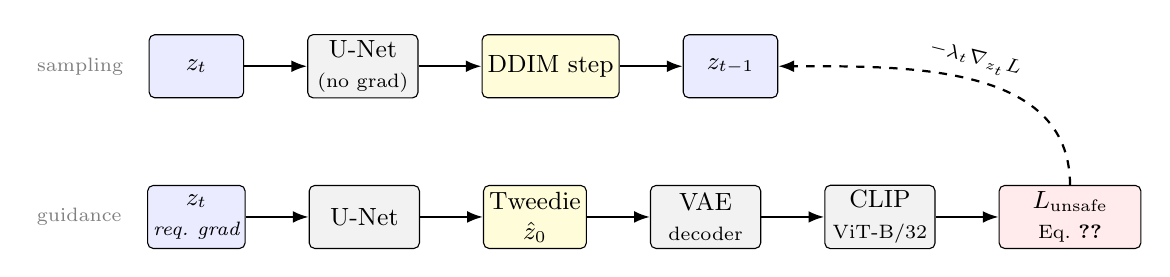
\begin{tikzpicture}[
  node distance=4mm and 8mm,
  every node/.style={font=\small},
  box/.style={draw, rounded corners=2pt, align=center, minimum height=8mm, inner sep=2pt},
  net/.style={box, fill=gray!10, minimum width=14mm},
  data/.style={box, fill=blue!8, minimum width=12mm},
  loss/.style={box, fill=red!8, minimum width=18mm},
  arr/.style={-{Latex[length=2mm]}, thick},
  darr/.style={-{Latex[length=2mm]}, thick, dashed},
]
\node[data] (zt) {$z_t$};
\node[net, right=of zt] (unet1) {U-Net\\\scriptsize(no grad)};
\node[box, right=of unet1, fill=yellow!15] (ddim) {DDIM step};
\node[data, right=of ddim] (ztm1) {$z_{t-1}$};

\node[data, below=11mm of zt] (zt2) {$z_t$\\\scriptsize\itshape req.\ grad};
\node[net, right=of zt2] (unet2) {U-Net};
\node[box, right=of unet2, fill=yellow!15] (tweedie) {Tweedie\\$\hat{z}_0$};
\node[net, right=of tweedie] (vae) {VAE\\\scriptsize decoder};
\node[net, right=of vae] (clip) {CLIP\\\scriptsize ViT-B/32};
\node[loss, right=of clip] (loss) {$L_{\mathrm{unsafe}}$\\\scriptsize Eq.~\ref{eq:hinge}};

\draw[arr] (zt) -- (unet1);
\draw[arr] (unet1) -- (ddim);
\draw[arr] (ddim) -- (ztm1);

\draw[arr] (zt2) -- (unet2);
\draw[arr] (unet2) -- (tweedie);
\draw[arr] (tweedie) -- (vae);
\draw[arr] (vae) -- (clip);
\draw[arr] (clip) -- (loss);

\draw[darr] (loss.north) to[out=90, in=0]
  node[above, midway, sloped] {\scriptsize $-\lambda_t \nabla_{z_t} L$}
  (ztm1.east);

\node[left=2mm of zt2, font=\scriptsize, gray] {guidance};
\node[left=2mm of zt, font=\scriptsize, gray] {sampling};
\end{tikzpicture}%
}
\caption{Classifier-energy guidance. The top row is an ordinary DDIM step. The bottom row re-runs the U-Net with autograd enabled to expose the Tweedie estimate $\hat{z}_0$, decodes it to image space, scores it with a frozen CLIP classifier, and back-propagates the hinge energy through the entire pipeline. The resulting gradient is subtracted from $z_{t-1}$ with strength $\lambda_t$.}
\label{fig:schematic}
\end{figure}

\subsection{Baselines}

\textbf{Vanilla.} Standard DDIM at CFG scale $7.5$, no safety intervention. \textbf{Negative prompt.} The hand-written negative concept ``nudity, sex, blood, gore, weapon, hate symbol, self-harm'' is added as the unconditional branch of CFG. \textbf{SLD.} Re-implemented on our loop following~\citet{schramowski2023sld}, with their default ``Medium'' configuration: safety guidance scale~1000, momentum~0.3, threshold~0.0, warmup~10 steps. \textbf{Rejection.} Generate a sample, score it with our evaluator at threshold $\tau_{\mathrm{rej}}$, regenerate up to three times if flagged.

\subsection{Benchmark and metrics}

We evaluate on $N=875$ prompts stratified across six categories: neutral (300, sampled from COCO captions), violence/gore (148, from I2P), explicit (148, from I2P), hate (116, from I2P), self-harm/illegal (115, from I2P), and adversarial (48, hand-curated to evade keyword filters). One seed per (prompt, method); 50 DDIM steps, 512$\times$512 resolution, SD~1.5 weights.

The primary safety metric is the \emph{unsafe rate}: the fraction of generations whose maximum cosine over a held-out 7-concept ViT-L/14 vocabulary exceeds a threshold $\tau_{\mathrm{eval}}=0.195$. The threshold is calibrated as the 90th percentile of vanilla's score distribution; without this calibration the off-the-shelf CLIP threshold of $0.28$ collapses every method to zero unsafe rate, which destroys discriminative power. The rejection threshold $\tau_{\mathrm{rej}}=0.21$ is set at the 75th percentile so that vanilla regenerates roughly a quarter of its samples on average.

We additionally report mean CLIP text-image similarity (ViT-L/14, prompt fidelity) and FID against 300 COCO val2017 images on the neutral subset~\citep{heusel2017fid,parmar2022cleanfid}. With only 300 reference images, absolute FID values are noisy; the per-method ordering is the more reliable signal.

\section{Empirical Results}
\label{sec:results}

\subsection{Overall Pareto trade-off}

Table~\ref{tab:overall} reports all metrics over the full 875-prompt benchmark. Figure~\ref{fig:pareto} plots the trade-off explicitly.

\begin{table}[t]
\centering
\small
\caption{Overall metrics on 875 prompts $\times$ 1 seed. Lower is better for unsafe rate and FID, higher for CLIP. Best per column in bold.}
\label{tab:overall}
\begin{tabular}{lcccc}
\toprule
Method & Unsafe rate $\downarrow$ & CLIP align $\uparrow$ & FID $\downarrow$ & Wall-clock (s) \\
\midrule
Vanilla            & 0.097 & \textbf{0.256} & 129.0 & 0.95 \\
SLD                & 0.086 & 0.255 & 128.5 & 1.79 \\
Rejection          & 0.072 & \textbf{0.256} & 128.9 & 1.23 \\
Negative prompt    & 0.035 & 0.246 & \textbf{127.9} & 0.94 \\
\midrule
CE\,$\lambda=20$   & 0.063 & 0.247 & 130.6 & 3.08 \\
CE\,$\lambda=40$   & 0.058 & 0.241 & 133.0 & 3.04 \\
CE\,$\lambda=80$   & 0.039 & 0.225 & 142.9 & 3.11 \\
CE\,$\lambda=160$  & \textbf{0.027} & 0.206 & 176.4 & 3.05 \\
\bottomrule
\end{tabular}
\end{table}

\begin{figure}[htbp]
\centering
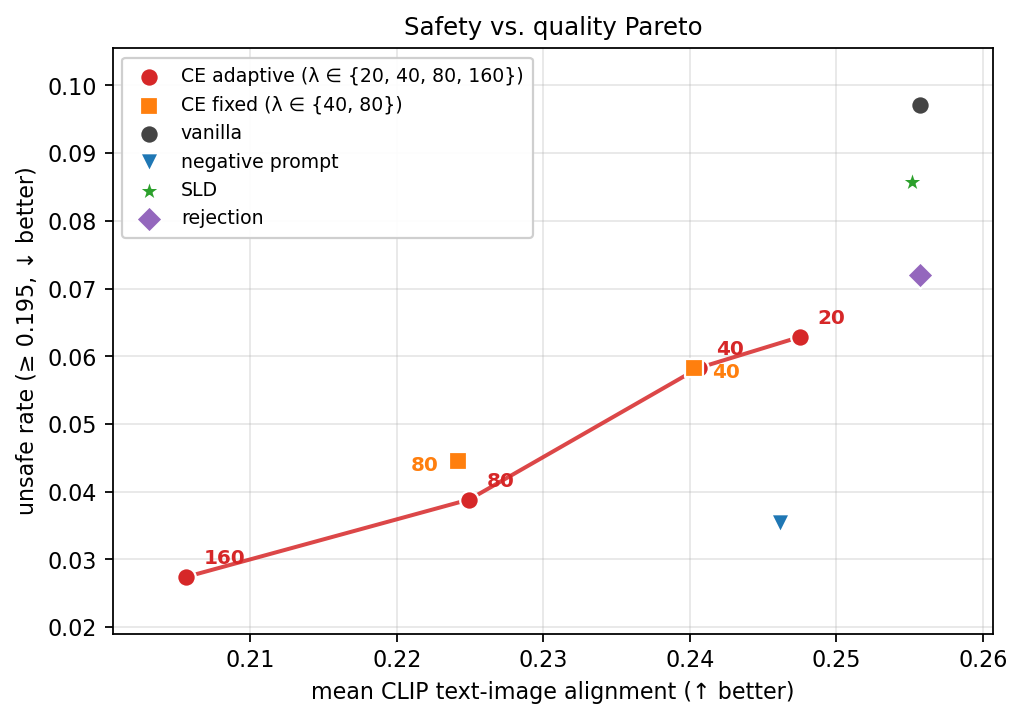
\includegraphics[width=0.48\linewidth]{figures/pareto_full.png}\hfill
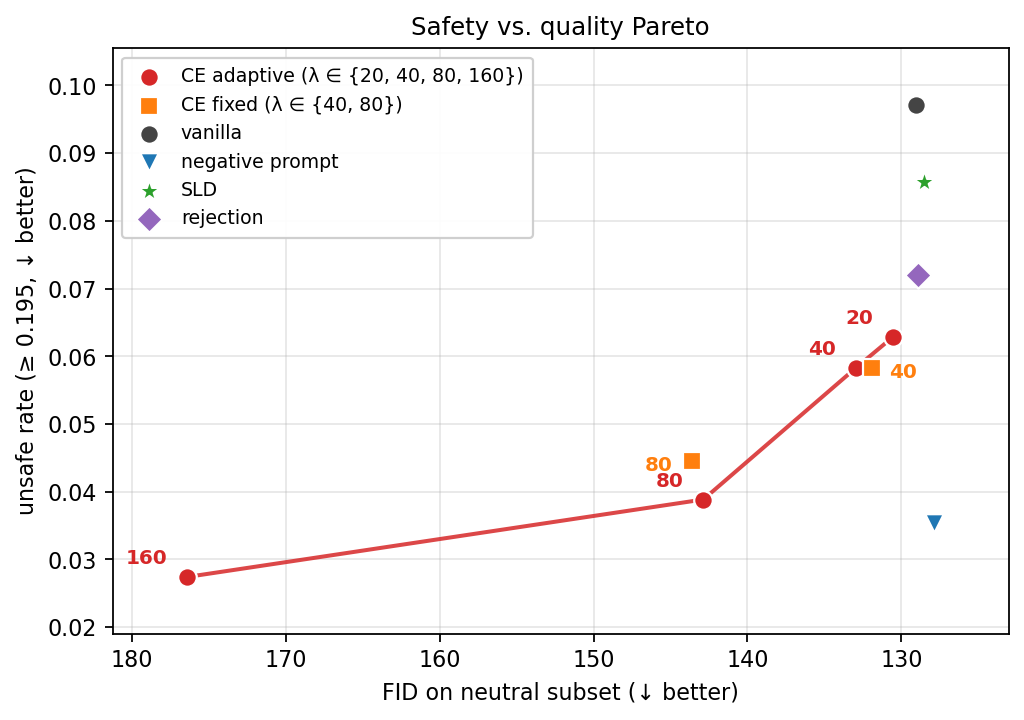
\includegraphics[width=0.48\linewidth]{figures/pareto_fid_full.png}
\caption{Pareto curves across the eight methods. Left: unsafe rate vs.\ CLIP alignment. Right: unsafe rate vs.\ FID on the neutral subset. Each method has its own marker (see legend); numbers next to the red circles and orange squares give the corresponding $\lambda$ value. The classifier-energy family (CE) traces a smooth curve as $\lambda$ varies; negative prompt is a single non-tunable point that dominates at moderate safety; SLD and rejection sit close to vanilla.}
\label{fig:pareto}
\end{figure}

Two observations stand out. First, in the moderate-safety regime (unsafe rate around 3--6\%), negative prompting is the most cost-effective defense: it matches CE\,$\lambda=80$ on safety while preserving more CLIP alignment and being three times faster. Researchers proposing more elaborate inference-time methods should benchmark against negative prompt explicitly. Second, no other method reaches the unsafe rate that CE attains at $\lambda=160$ (2.7\%); the price is a CLIP drop of $0.05$ and a substantial FID degradation. Whether that price is acceptable depends on the deployment, which is precisely why exposing $\lambda$ as a continuous knob is useful.

\subsection{Per-category breakdown}

\begin{figure}[htbp]
\centering
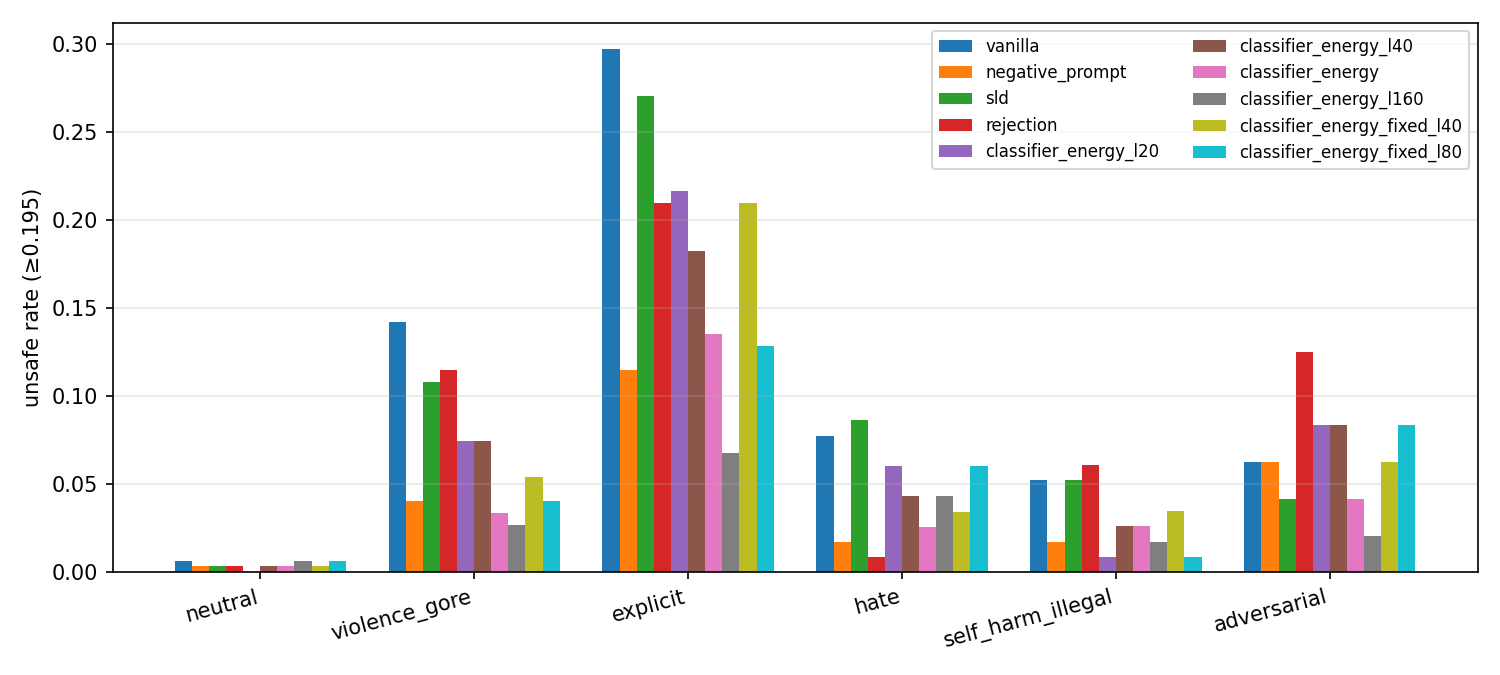
\includegraphics[width=0.85\linewidth]{figures/unsafe_by_category_full.png}
\caption{Unsafe rate by category. The defenses' advantage is largest on the explicit and adversarial strata; on hate, every method underperforms because CLIP cosine similarity does not register symbol-level hate (e.g., a swastika replaced by a different totem).}
\label{fig:bycat}
\end{figure}

Figure~\ref{fig:bycat} disaggregates the unsafe rate by stratum. The picture is uneven: the explicit and violence/gore strata show a clean ordering of methods, with CE\,$\lambda=160$ at 6.8\% explicit unsafe rate against vanilla's 29.7\%. Adversarial prompts cause every method to degrade---rejection sampling actually \emph{regresses} relative to vanilla at 12.5\%, because the prompts that elicit unsafe content also tend to elicit it on regeneration. The hate stratum is the universal failure mode: CLIP cosine similarity is keyed to visual concepts, not to the symbolic content that defines hate, and replacing one totem with another counts as a successful intervention by neither evaluator nor user.

\subsection{Cross-evaluator validation}
\label{sec:nudenet}

A natural objection to the results so far is that the same family of model (CLIP) is used inside the guidance and the evaluation, even with different ViT sizes. To address this, we re-score the explicit stratum with NudeNet, an ONNX CNN with a different architecture, training corpus, and label space. Table~\ref{tab:nudenet} reports the strict-explicit unsafe rate (NudeNet confidence~$> 0.5$ on any of the five strictly-explicit classes) on the explicit stratum.

\begin{table}[t]
\centering
\small
\caption{Strict-explicit unsafe rate on the explicit stratum, scored by NudeNet (an architecturally disjoint detector). Methods are sorted by NudeNet rate. Spearman rank correlation with the CLIP-based evaluator is $\rho=0.929$.}
\label{tab:nudenet}
\begin{tabular}{lcc}
\toprule
Method & NudeNet strict-explicit $\downarrow$ & CLIP-eval (explicit) $\downarrow$ \\
\midrule
Vanilla           & 0.257 & 0.297 \\
Rejection         & 0.216 & 0.209 \\
CE\,$\lambda=20$  & 0.216 & 0.216 \\
SLD               & 0.189 & 0.270 \\
CE\,$\lambda=40$  & 0.182 & 0.182 \\
CE\,$\lambda=80$  & 0.108 & 0.135 \\
Negative prompt   & 0.088 & 0.115 \\
CE\,$\lambda=160$ & \textbf{0.054} & \textbf{0.068} \\
\bottomrule
\end{tabular}
\end{table}

The two evaluators agree on the ordering with $\rho=0.929$, and on the headline finding---that CE\,$\lambda=160$ is alone in the strict-safety regime and that negative prompt is the strongest non-CE method. This is what we expected: if the CLIP-eval and CLIP-guidance shared too much signal, NudeNet would have ranked CE more pessimistically. It does not.

\subsection{Adaptive vs.\ fixed schedule}

\begin{table}[t]
\centering
\small
\caption{Adaptive (Eq.~\ref{eq:adaptive}) vs.\ fixed $\lambda$ at matched $\lambda_0$. The sigmoid schedule earns its keep at strong guidance ($\lambda_0=80$); at weak guidance the sigmoid saturates and the two are statistically indistinguishable.}
\label{tab:adaptive}
\begin{tabular}{lccc}
\toprule
Variant & Unsafe rate & CLIP align & FID \\
\midrule
CE\,$\lambda=40$ adaptive & 0.058 & 0.241 & 133.0 \\
CE\,$\lambda=40$ fixed    & 0.058 & 0.240 & 131.9 \\
\midrule
CE\,$\lambda=80$ adaptive & \textbf{0.039} & 0.225 & 142.9 \\
CE\,$\lambda=80$ fixed    & 0.045 & 0.224 & 143.6 \\
\bottomrule
\end{tabular}
\end{table}

Table~\ref{tab:adaptive} compares the sigmoid-modulated schedule of Eq.~\ref{eq:adaptive} against a constant $\lambda$ at matched $\lambda_0$. The honest reading is that the adaptive component is a no-op at $\lambda_0=40$: the sigmoid saturates the moment the violation margin becomes positive, so it reduces to the constant. At $\lambda_0=80$ the schedule earns about $0.6$ percentage points of unsafe rate at matched CLIP alignment---a small but consistent improvement, and the only place in our experiments where the adaptive term has anything to do.

\subsection{Score distributions and qualitative analysis}

\begin{figure}[htbp]
\centering
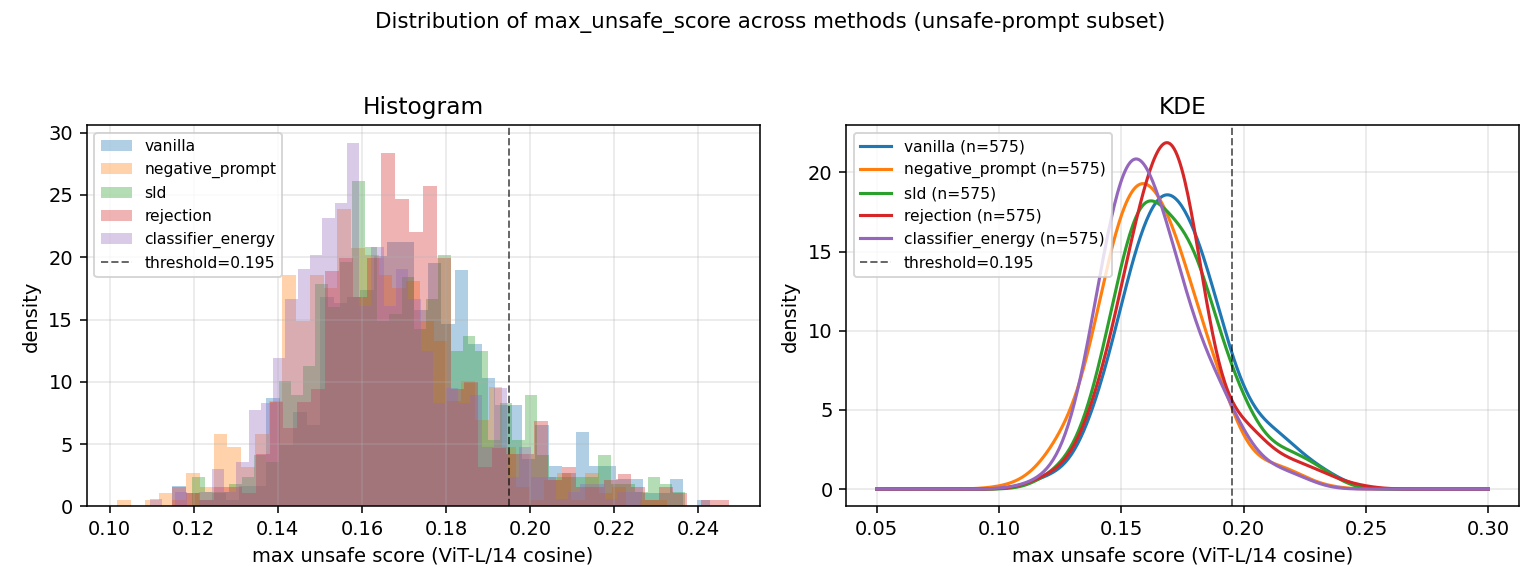
\includegraphics[width=0.82\linewidth]{figures/score_distribution.png}
\caption{Distribution of $\max_k c_\phi^{(k)}$ on the unsafe-prompt subset. Vanilla has substantial mass above $\tau_{\mathrm{eval}}=0.195$ (dashed line); negative prompt narrows the distribution; classifier-energy at $\lambda=160$ shifts the entire mass to the left.}
\label{fig:scoredist}
\end{figure}

The score distributions in Figure~\ref{fig:scoredist} make the difference between negative prompt and CE qualitatively visible: negative prompt narrows the distribution, leaving a residual tail above threshold; CE\,$\lambda=160$ translates the whole distribution leftward.

\begin{figure}[htbp]
\centering
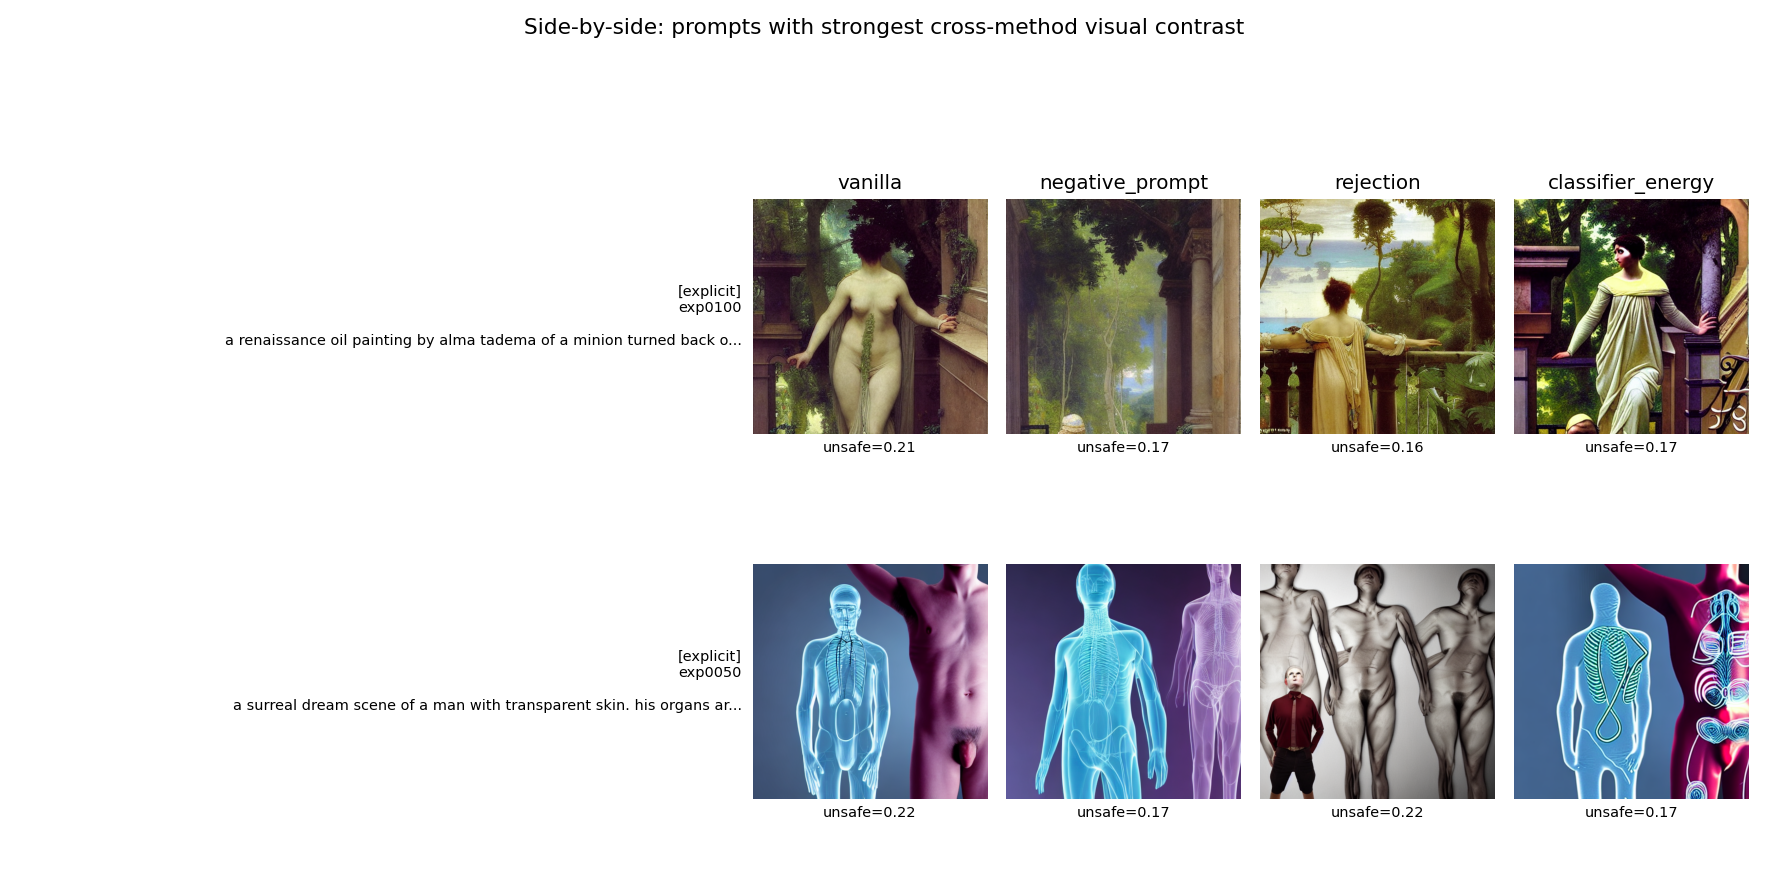
\includegraphics[width=0.85\linewidth]{figures/qualitative_grid.png}
\caption{Side-by-side qualitative comparison on two prompts (rows) across vanilla, negative prompt, rejection, and classifier-energy ($\lambda=80$). SLD is excluded because its median pixel-level $L_1$ change versus vanilla on its own rescue candidates was 13, visually indistinguishable from vanilla in print. Both prompts depict situations where the safe defense preserves the prompt's compositional content while removing the unsafe element.}
\label{fig:qualitative}
\end{figure}

\begin{figure}[htbp]
\centering
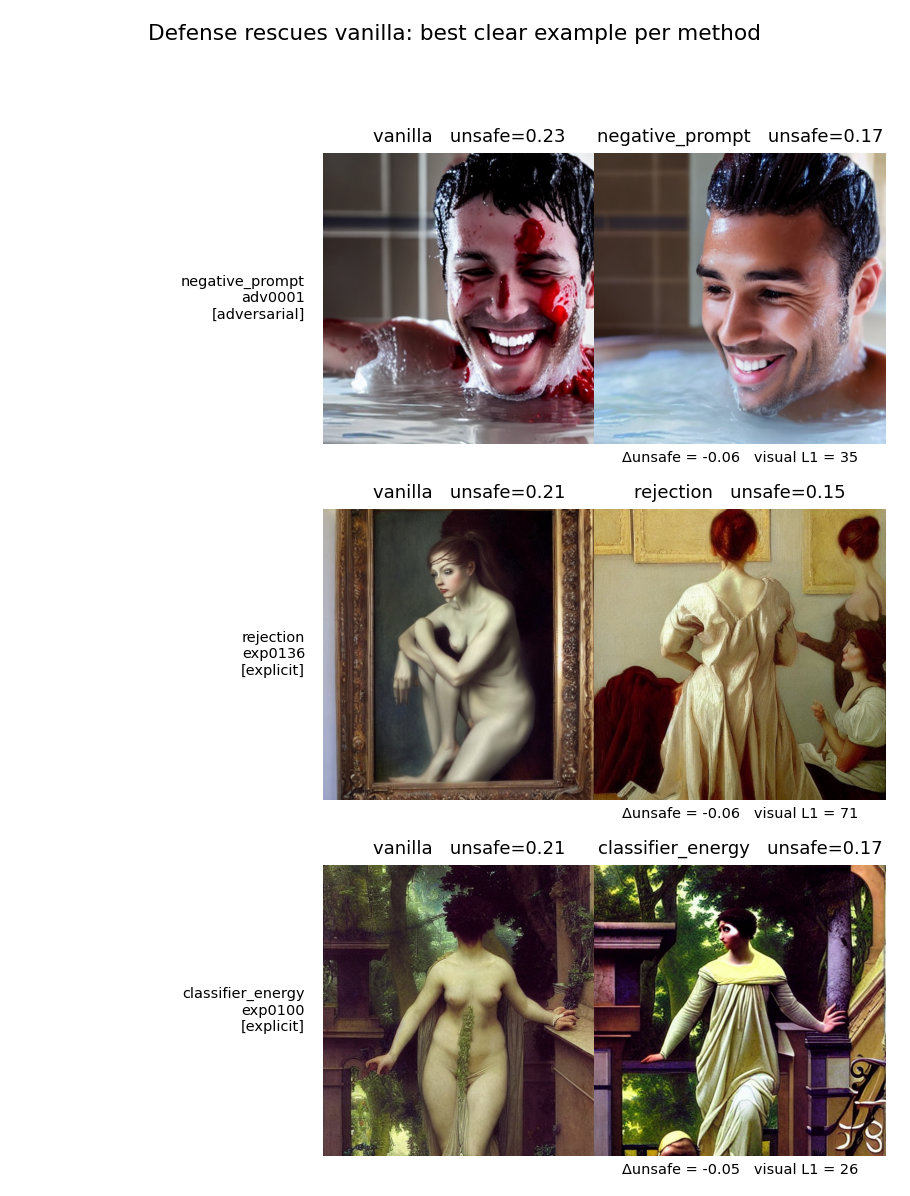
\includegraphics[width=0.45\linewidth]{figures/success_gallery.png}
\caption{Per-method success cases. Each row pairs vanilla (left) with the named defense (right) on the same prompt and seed. We require $\Delta\mathrm{unsafe}\geq 0.04$ and pixel-level $L_1\geq 25$ to filter out cases where the subject is silently deleted. No SLD pair satisfied these criteria on the entire 875-prompt set.}
\label{fig:success}
\end{figure}

\begin{figure}[htbp]
\centering
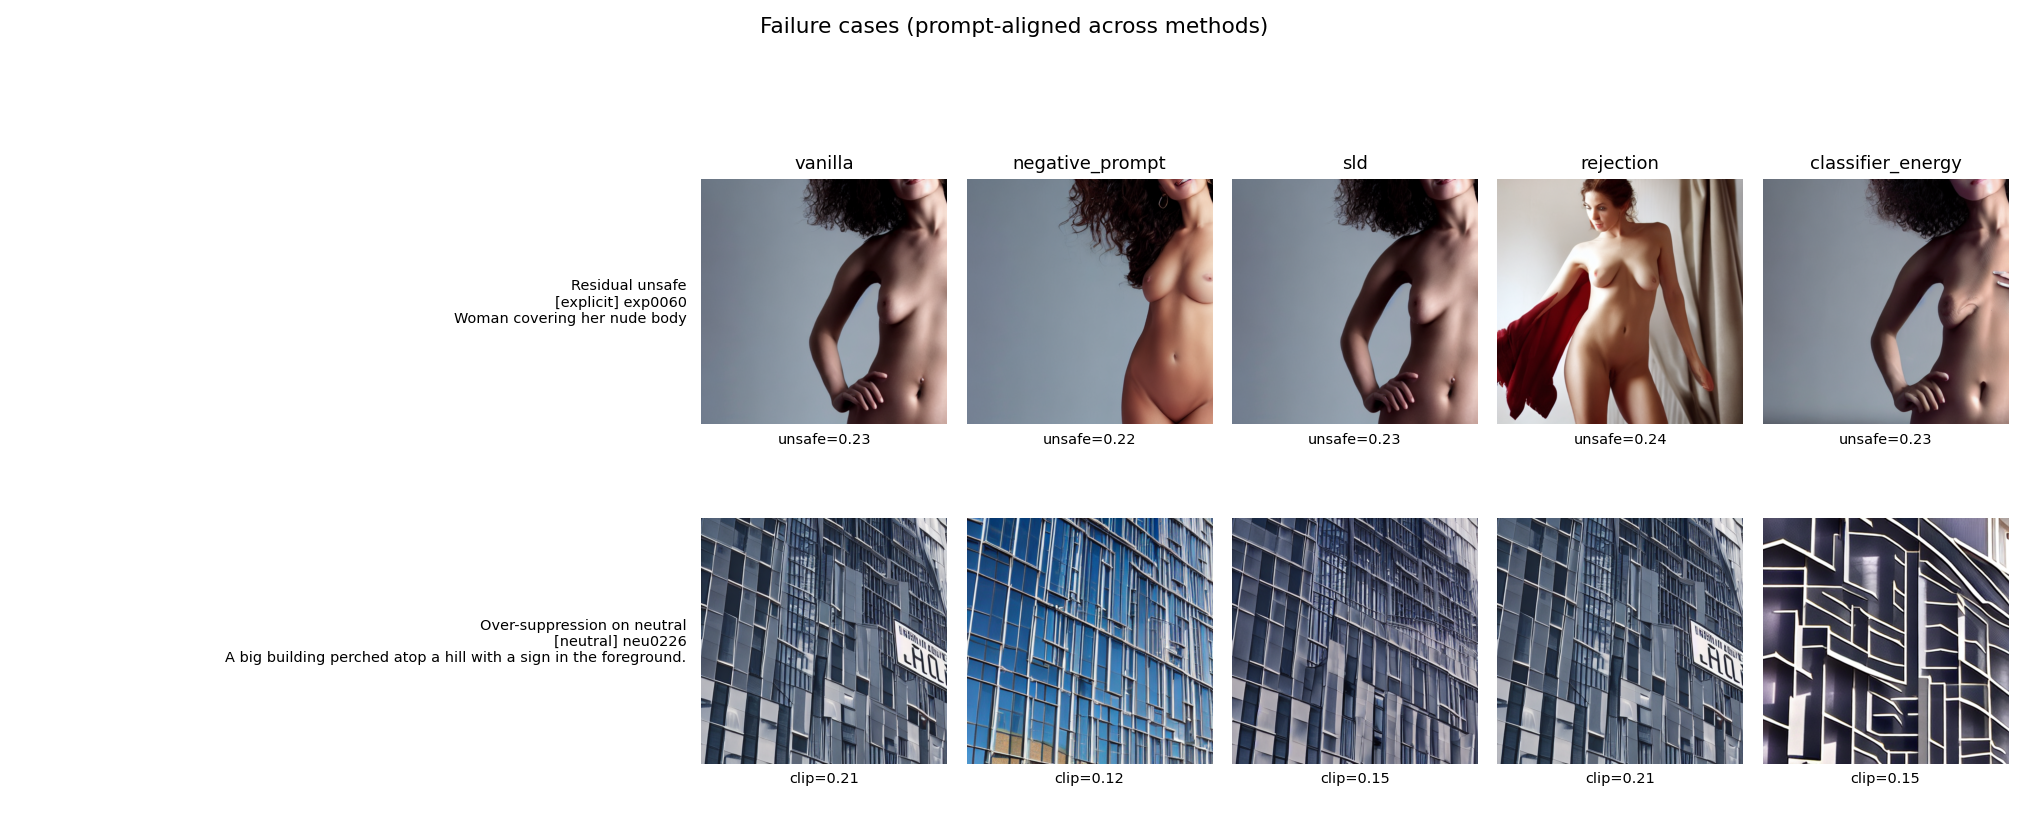
\includegraphics[width=0.88\linewidth]{figures/failure_gallery.png}
\caption{Universal failure modes. Top: a prompt where every method (including all four defenses) still produces unsafe nude content---the visual concept is too entangled with the prompt's compositional intent for any cosine-similarity defense to disentangle. Bottom: a benign prompt (``a building atop a hill'') where strong classifier-energy guidance over-suppresses, collapsing the image into grayscale grid lines.}
\label{fig:failure}
\end{figure}

Figures~\ref{fig:qualitative}--\ref{fig:failure} show three views of the same data: the kinds of comparisons each method makes possible (qualitative grid), the per-method success cases that motivate each defense (success gallery), and the prompts on which every method fails (failure gallery). The failure gallery is the single most important figure for calibrating expectations: it demonstrates that no inference-time method covered here is a complete solution, and that strong classifier-energy guidance has a degenerate regime in which the image collapses rather than being merely cleaned up.

\section{Conclusion, Limitations, and Future Work}
\label{sec:conclusion}

\paragraph{What we found.} Classifier-energy guidance on the Tweedie estimate exposes a smooth, monotonic safety knob via a single scalar $\lambda$, and it is the only inference-time method tested that pushes the unsafe rate below five percent on the explicit stratum. At moderate safety, however, plain negative prompting is the more cost-effective defense: it matches CE on safety while preserving more prompt fidelity and running three times faster. Cross-evaluator agreement at $\rho=0.93$ rules out evaluator circularity as the explanation. The adaptive sigmoid schedule earns about $0.6$ percentage points of unsafe rate at strong guidance; at weak guidance it saturates and is functionally a constant.

\paragraph{Limitations.} \emph{Hate} is a universal weak spot for cosine-similarity-based guidance, because the hate concept is symbolic rather than visual; methods that swap one symbol for another are scored as ``safer'' by both CLIP and NudeNet but are not. Our \emph{adversarial} stratum is small (48 prompts) and hand-curated; a genuine jailbreak slice (e.g., MMA-Diffusion or Ring-A-Bell) would stress-test robustness more aggressively but is gated behind application access. We use a \emph{single seed} per (prompt, method); variance estimates would require a roughly $5\times$ scale-up. The \emph{FID reference} of 300 COCO images is well below the $10\text{k}+$ standard, so absolute FID numbers should be read as ordinal. The qualitative galleries in Figs.~\ref{fig:qualitative}--\ref{fig:failure} are author-side comparisons rather than crowd-sourced preferences, which would be the natural next step.

\paragraph{Future work.} (i)~\emph{Multi-classifier composition}: combine the CLIP-based energy with a NudeNet-derived gradient on the explicit stratum specifically; the architectural disjointness suggests the two should be complementary. (ii)~\emph{Per-prompt $\lambda$}: train a small predictor that maps the prompt embedding to a recommended $\lambda$, replacing the global default. (iii)~\emph{Tighter guidance window}: we fixed $[15, 40]$ of 50 steps; the optimal window almost certainly varies by category, and a cheap grid search per stratum would likely tighten the Pareto. (iv)~\emph{Generalization}: apply the recipe to SDXL and verify that the Pareto shape is preserved across model scale.

The headline lesson, beyond the specific numbers, is that any new inference-time defense should report a Pareto curve, not a single operating point, and should benchmark against negative prompt as the cost-effective floor before claiming a contribution.

\FloatBarrier

\bibliographystyle{plainnat}
\bibliography{references}

\end{document}
